% Provenance (never printed): see sources/outline_sources.md (Year 3: gravitational
% potential, spherical harmonics, J2, reference ellipsoid, geoid, satellite gravimetry,
% flexure of the lithosphere). Brief: sources/book5/BRIEFS.md, ch. 3. Curves from
% figdata/bachelor-3/hydrostatic_figure.py, ice_mass.py (IMBIE 2021), flexure.py.
% Exercise and problem values in the Book 5 scratch calculator calc/ch03.py.
\chapter{गुरुत्व और पृथ्वी की आकृति}\label{ch:b3:gravity-geodesy}

दो उपग्रह पृथ्वी की परिक्रमा एक के पीछे एक करते हैं,
\qty{500}{km} से अधिक ऊँचाई पर और लगभग \qty{220}{km} की दूरी पर,
और उनके बीच की दूरी हर समय मापते हैं, एक माइक्रोमीटर के भीतर।
% ledger: geod5:grace, geod5:grace-ranging
जब वे ऐसे किसी स्थान के ऊपर से गुजरते हैं जहाँ द्रव्यमान संकेंद्रित है, तो आगे वाला उपग्रह पहले आगे खिंचता है
और दूरी बढ़ती है; फिर पीछे वाला उपग्रह बारी-बारी से खिंचता है और दूरी घटती है।
इन सूक्ष्म परिवर्तनों से, 2002 से हर महीने, पृथ्वी के गुरुत्व क्षेत्र का
मानचित्र उसके बदलने के साथ बनाया गया है: नदी-द्रोणियों में संचित जल
ऋतुओं के साथ ऊपर-नीचे होता है, और ग्रीनलैंड तथा अंटार्कटिका की विशाल हिमचादरें
वर्ष-दर-वर्ष द्रव्यमान खो रही हैं। गुरुत्व वह तौलता है जिसे आँख
देख नहीं सकती। इस अध्याय में घूमते ग्रह का गुरुत्व क्षेत्र उसके विभव से
निर्मित किया जाता है, उसमें से चपटापन और जड़त्व आघूर्ण ज्ञात होते हैं,
गुरुत्व की विसंगतियाँ कक्षा तक अनुसरित की जाती हैं, और फिर सतह पर जो
गुरुत्व प्रकट करता है, उनमें से एक की ओर मुड़ा जाता है: किसी ज्वालामुखी के भार के नीचे \omterm{def:b3:gravity-geodesy:flexure}{स्थलमंडलीय आनमन}।

\begin{recall}
न्यूटन का गुरुत्वाकर्षण नियम, गुरुत्वीय स्थितिज ऊर्जा और
घूर्णन फ़्रेम में अपकेंद्री बल भौतिकी की पुस्तकों में हैं; ठोस के जड़त्व आघूर्ण
और लीजेंड्र बहुपद $P_2(x) = (3x^2 - 1)/2$ भौतिकी और गणित की
पुस्तकों के विश्वविद्यालयी खंडों में हैं, यंग मापांक $E$ और
पॉइसन अनुपात $\nu$ भौतिकी की पुस्तकों के स्नातक वर्ष 3 खंड में हैं। भूगणित और
दीर्घवृत्तज का चपटापन $f = (a - b)/a$, जिसके अर्ध-अक्ष $a > b$ हैं, कक्षा 10 में
परिचित हुए थे। समस्थिति, एरी प्रतिपूर्ति, सामान्य गुरुत्व, भूआभ, जियॉइड
ऊँचाई और गुरुत्व विसंगतियाँ पुस्तक 3 (स्नातक वर्ष 1) में, उसके
समस्थिति और गुरुत्व विसंगतियों वाले अध्याय में परिभाषित की गई थीं।
\end{recall}

\section{भू-विभव}

घूमते हुए ग्रह पर स्थिर पिंड ग्रह के द्रव्यमान का आकर्षण अनुभव करता है
और उसके साथ घूमते फ़्रेम में अपकेंद्री बल भी। दोनों एक
विभव से निकलते हैं।

\begin{definition}[भू-विभव]\label{def:b3:gravity-geodesy:geopotential}
\emph{भू-विभव}\index{भू-विभव} प्रति एकांक द्रव्यमान की वह स्थितिज ऊर्जा है
जो कोणीय वेग $\omega$ से पृथ्वी के साथ घूमते फ़्रेम में, गुरुत्वाकर्षण
और अपकेंद्री बल दोनों की मिलकर होती है:
\[
  W(\mathbf r) = V(\mathbf r) + \Phi(\mathbf r),\qquad
  V(\mathbf r) = -G\int_{\text{पृथ्वी}}\frac{\mathrm dm'}{|\mathbf r - \mathbf r'|},\qquad
  \Phi(\mathbf r) = -\tfrac12\omega^2 s^2,
\]
जहाँ $s$ घूर्णन अक्ष से दूरी है और गुरुत्व
$\mathbf g = -\nabla W$ है, और $W = \text{स्थिरांक}$ वाले पृष्ठ इसके
स्तर-पृष्ठ हैं: गुरुत्व हर जगह उन पर लंबवत होता है।
\end{definition}

ओलंब रेखा $-\nabla W$ के अनुदिश लटकती है, और स्थिर जल एक स्तर-पृष्ठ पर
ठहरता है। इसलिए घूमता तरल ग्रह अपने ही किसी स्तर-पृष्ठ का आकार ले लेता है:
अपकेंद्री विभव, जो भूमध्य रेखा पर सबसे गहरा होता है, उसे फुला देता है
और ध्रुवों को चपटा कर देता है।

\begin{omfigure}
\begin{tikzpicture}[font=\small, x=1cm, y=1cm]
\draw[gray, densely dashed] (0,0) circle (2.4);
\draw[very thick, blue!60!black] (0,0) ellipse (2.75 and 2.1);
\draw[->, thick] (0,-2.7) -- (0,2.9) node[above] {घूर्णन अक्ष};
\draw[gray] (-3.2,0) -- (3.2,0);
\fill (0,0) circle (1.6pt);
% a point at latitude 40 deg (parameter) on the ellipse; the attraction points at
% the centre, the centrifugal force is horizontal, and their sum is drawn along the
% inward normal of the ellipse: lengths solved so that the sum is normal (calc/ch03_fig.py)
\coordinate (P) at (2.107,1.350);
\fill (P) circle (1.8pt);
\draw[->, thick, red!70!black] (P) -- (1.012,0.650);
\node[font=\scriptsize, red!70!black, anchor=south east] at (1.50,1.02) {आकर्षण};
\draw[->, thick, orange!80!black] (P) -- (2.565,1.350) node[right, font=\scriptsize] {अपकेंद्री};
\draw[gray, densely dotted] (1.012,0.650) -- (1.470,0.650);
\draw[->, very thick, green!45!black] (P) -- (1.470,0.650);
\node[font=\scriptsize, green!45!black, anchor=north] at (1.470,0.600) {गुरुत्व};
\node[blue!60!black, anchor=west, font=\scriptsize] at (2.4,-1.7) {स्तर-पृष्ठ};
\node[gray!40!black, anchor=east, font=\scriptsize] at (-1.9,-2.2) {गोला};
\end{tikzpicture}

\par\smallskip{\small घूमते ग्रह का एक स्तर-पृष्ठ (योजनाबद्ध, चपटापन बहुत
बढ़ाकर दिखाया गया है)। हर बिंदु पर गुरुत्व, यानी आकर्षण और अपकेंद्री बल का
योग, स्तर-पृष्ठ पर लंबवत होता है; वह केंद्र की ओर नहीं इंगित करता,
सिवाय ध्रुवों और भूमध्य रेखा पर।}
\label{fig:b3:gravity-geodesy:equipotential}
\end{omfigure}

ग्रह के बाहर गुरुत्वीय विभव लाप्लास समीकरण का पालन करता है, और
उसके अनंत पर नियमित हल ठोस गोलीय हार्मोनिक होते हैं।

\begin{proposition}[भू-विभव का गोलीय-हार्मोनिक प्रसार]\label{prop:b3:gravity-geodesy:harmonics}
द्रव्यमान $M$ और विषुवतीय त्रिज्या $a$ वाले पिंड के बाहर, मूल बिंदु उसके
द्रव्यमान-केंद्र पर और $z$ अक्ष उसके घूर्णन अक्ष के अनुदिश हो, तो गुरुत्वीय
विभव दूरी $r$, सहअक्षांश $\theta$ और देशांतर $\lambda$ पर इस प्रकार है:
\begin{multline*}
  V = -\frac{GM}{r}\Biggl[1 - \sum_{n=2}^{\infty}\left(\frac ar\right)^nJ_nP_n(\cos\theta)\\
  + \sum_{n=2}^{\infty}\sum_{m=1}^{n}\left(\frac ar\right)^nP_{nm}(\cos\theta)
  (C_{nm}\cos m\lambda + S_{nm}\sin m\lambda)\Biggr],
\end{multline*}
जहाँ $P_n$ लीजेंड्र बहुपद और $P_{nm}$ संबद्ध फलन हैं; गुणांक
$J_n$, $C_{nm}$, $S_{nm}$ प्रेक्षणों से निर्धारित की गई संख्याएँ हैं। किसी
अक्ष-सममित पिंड के लिए केवल ज़ोनल पद $J_n$ शेष रहते हैं। कोटि 1 का
कोई पद नहीं आता।
\end{proposition}

\begin{proof}
गोलीय निर्देशांकों में लाप्लास समीकरण का चर-पृथक्करण
अनंत पर नियमित हल $r^{-(n+1)}P_{nm}(\cos\theta)e^{\pm
im\lambda}$ देते हैं (गणित की पुस्तकों के विश्वविद्यालयी खंड); पिंडों के बाहर का कोई भी विभव
इन्हीं का योग होता है। कोटि 0 का पद $-GM/r$ है, जो
पूरे द्रव्यमान का विभव है। कोटि-1 के पद प्रथम आघूर्णों के समानुपाती होते हैं,
$\int\mathbf r'\,\mathrm dm'$, जो शून्य हो जाते हैं जब मूल बिंदु द्रव्यमान-केंद्र पर हो।
अक्षीय सममिति हर उस पद को हटा देती है जो $\lambda$ पर निर्भर करता है।
\end{proof}

\begin{definition}[गतिक रूप-गुणक]\label{def:b3:gravity-geodesy:j2}
\emph{गतिक रूप-गुणक}\index{गतिक रूप-गुणक} किसी ग्रह का $J_2$
उसके दूसरे कोटि के मंडलीय हार्मोनिक का गुणांक है: उसके बाहरी विभव का
गोले के विभव से सबसे बड़ा विचलन, जो उसके चपटेपन से उत्पन्न होता है। पृथ्वी के लिए
$J_2 = \num{1.08263e-3}$ है।
% ledger: geod5:grs80-defining
\end{definition}

\begin{theorem}[मैककला सूत्र]\label{thm:b3:gravity-geodesy:maccullagh}
मान लीजिए $A$, $B$, $C$ द्रव्यमान $M$ के पिंड के मुख्य जड़त्व आघूर्ण हैं,
उसके द्रव्यमान-केंद्र से होकर जाने वाली अक्षों के सापेक्ष, और $I$ उसका जड़त्व आघूर्ण
द्रव्यमान-केंद्र से किसी बाहरी बिंदु की ओर जाने वाली रेखा के सापेक्ष है, जिसकी दूरी $r$ है। 
$r^{-3}$ की कोटि तक उस बिंदु पर गुरुत्वीय विभव
\emph{मैककला सूत्र}\index{मैककला सूत्र} द्वारा दिया जाता है
\[
  V = -\frac{GM}{r} - \frac{G(A + B + C - 3I)}{2r^3} .
\]
$z$ अक्ष के परितः सममित पिंड के लिए ($A = B$),
$V = -\dfrac{GM}{r} + \dfrac{G(C - A)}{r^3}P_2(\cos\theta)$ है, अतः
\[
  J_2 = \frac{C - A}{Ma^2} .
\]
\end{theorem}

\begin{proof}
$\hat{\mathbf r}$ को बिंदु की ओर का एकक सदिश और $r' \ll r$ मानते हुए,
\[
  \frac{1}{|\mathbf r - \mathbf r'|} = \frac1r + \frac{\hat{\mathbf r}\cdot\mathbf r'}{r^2}
  + \frac{3(\hat{\mathbf r}\cdot\mathbf r')^2 - r'^2}{2r^3} + O(r^{-4}).
\]
द्रव्यमान पर समाकलन करने पर पहला पद $M/r$ देता है और दूसरा शून्य हो जाता है
(द्रव्यमान-केंद्र)। तीसरे के लिए, $\int r'^2\,\mathrm dm' = (A + B + C)/2$ है, क्योंकि
$A + B + C = \int 2r'^2\,\mathrm dm'$ है, और $\int(\hat{\mathbf r}\cdot\mathbf
r')^2\,\mathrm dm' = \int r'^2\,\mathrm dm' - I$ है, क्योंकि रेखा से दूरी का वर्ग
$r'^2 - (\hat{\mathbf r}\cdot\mathbf r')^2$ है। कोष्ठक का समाकलन
$3(A + B + C)/2 - 3I - (A + B + C)/2 = A + B + C - 3I$ देता है। $A = B$ के लिए,
सह-अक्षांश $\theta$ पर स्थित रेखा के सापेक्ष आघूर्ण $I = A\sin^2\theta + C\cos^2\theta$ है,
और $2A + C - 3I = (C - A)(1 - 3\cos^2\theta) = -2(C - A)P_2(\cos\theta)$ है।
\cref{prop:b3:gravity-geodesy:harmonics} से तुलना करने पर
$J_2Ma^2 = C - A$ प्राप्त होता है।
\end{proof}

विभव का दूसरे कोटि का पद इसलिए जड़त्व आघूर्णों के अंतर को मापता है,
स्वयं आघूर्णों को नहीं। पृथ्वी की अक्ष का पुरस्सरण,
जो सूर्य और चंद्रमा के बल-आघूर्णों से उसके भूमध्यरेखीय उभार पर उत्पन्न होता है,
गतिक उत्केंद्रता $H = (C - A)/C$ को मापता है; $J_2$ और $H$ मिलकर
$C/(Ma^2)$ देते हैं, जो जड़त्व-आघूर्ण गुणक है और पृथ्वी के लिए \num{0.3308} है,
% ledger: earth:MoI
एकसमान गोले के \num{0.4} से यह काफ़ी कम है: द्रव्यमान
केंद्र की ओर संकेंद्रित है।

\section{घूर्णनशील दीर्घवृत्तज}

\begin{definition}[संदर्भ दीर्घवृत्तज]\label{def:b3:gravity-geodesy:ellipsoid}
\emph{संदर्भ दीर्घवृत्तज}\index{संदर्भ दीर्घवृत्तज} एक परिक्रमण दीर्घवृत्तज है,
जिसका भूमध्यरेखीय अर्ध-अक्ष $a$ और चपटापन $f$ है, और जिसे इस प्रकार चुना जाता है कि वह
स्वयं एक प्रतिरूप विभव का समविभव पृष्ठ हो, अर्थात एक घूर्णनशील पिंड का विभव जिसका
द्रव्यमान $M$, कोणीय वेग $\omega$ और पृथ्वी का \omterm{def:b3:gravity-geodesy:j2}{गतिक रूप-गुणक}
$J_2$ है। इसे परिभाषित करने वाले चार स्थिरांक हैं; भूगणितीय संदर्भ
प्रणाली 1980 इन्हें लेती है
\begin{gather*}
  a = \qty{6378137}{m},\qquad GM = \qty{3.986005e14}{m^3.s^{-2}},\\
  J_2 = \num{1.08263e-3},\qquad \omega = \qty{7.292115e-5}{rad.s^{-1}},
\end{gather*}
और इनसे चपटापन $f = \num{0.00335281068}$
($1/f = \num{298.257222}$) और अर्ध-लघु अक्ष
$b = \qty{6356752.3141}{m}$ निकालती है।
% ledger: geod5:grs80-defining, geod5:grs80-derived
\end{definition}

प्रतिरूप का विभव, जिसे सामान्य विभव कहते हैं, बंद रूप में ज्ञात है, और
दीर्घवृत्तज पर उसका गुरुत्व, यानी सामान्य गुरुत्व, भी इसी प्रकार ज्ञात है, जैसा पुस्तक 3 (स्नातक वर्ष 1) में बताया गया है।

\begin{proposition}[सोमिलियाना सूत्र]\label{prop:b3:gravity-geodesy:somigliana}
अर्ध-अक्षों $a$, $b$ वाले \omterm{def:b3:gravity-geodesy:ellipsoid}{संदर्भ दीर्घवृत्तज} पर, जहाँ भूमध्यरेखा पर सामान्य गुरुत्व
$\gamma_e$ और ध्रुवों पर $\gamma_p$ है, और भूगणितीय अक्षांश
$\varphi$ पर सामान्य गुरुत्व \emph{सोमिलियाना
सूत्र}\index{सोमिलियाना सूत्र} द्वारा दिया जाता है
\[
  \gamma(\varphi) = \frac{a\gamma_e\cos^2\varphi + b\gamma_p\sin^2\varphi}
  {\sqrt{a^2\cos^2\varphi + b^2\sin^2\varphi}} .
\]
भूगणितीय संदर्भ प्रणाली 1980 के लिए $\gamma_e = \qty{9.7803267715}{m.s^{-2}}$
और $\gamma_p = \qty{9.8321863685}{m.s^{-2}}$ है, और श्रेणी
$\gamma = 9.780327(1 + 0.0053024\sin^2\varphi - 0.0000058\sin^22\varphi)$
\unit{m.s^{-2}} सूत्र को \qty{0.1}{\milli\gal} की सीमा तक पुनरुत्पादित करती है।
% ledger: geod5:grs80-derived, moritz:grs80 (Book 3, read-only)
\end{proposition}
\admitted

घूर्णनशील ग्रह कितना चपटा होना चाहिए? यदि यह द्रवस्थैतिक साम्य में एक द्रव है,
तो इसका चपटापन उसके घूर्णन और इस पर निर्भर करता है कि उसका द्रव्यमान
गहराई में किस प्रकार वितरित है, इससे निश्चित होता है।

\begin{proposition}[क्लेरो और डार्विन--रेडाउ संबंध]\label{prop:b3:gravity-geodesy:clairaut}
द्रवस्थैतिक साम्य में एक ग्रह के लिए, $m = \omega^2a^2b/(GM)$ को
भूमध्यरेखा पर अपकेंद्री और गुरुत्वीय त्वरण का अनुपात मानते हुए,
$f$ और $m$ में प्रथम कोटि तक:
\[
  J_2 = \frac{2f - m}{3}\qquad\text{(क्लेरो)},\qquad
  \frac{C}{Ma^2} = \frac23\left[1 - \frac25\sqrt{\frac52\frac mf - 1}\right]
  \qquad\text{(डार्विन--रेडाउ)} .
\]
एकसमान ग्रह ($C/Ma^2 = 0.4$) के लिए $f = 5m/4$ है; वह ग्रह जिसका द्रव्यमान
केंद्र की ओर संकेंद्रित है, कम चपटा होता है।
\end{proposition}
\admitted

क्लेरो संबंध में पृथ्वी का $m = \num{0.00344979}$ रखने पर उसके मापे गए
$J_2$ से $f = \num{0.0033488}$, या $1/298.6$ मिलता है,
जो दीर्घवृत्तज के चपटेपन के \qty{0.12}{\percent} के भीतर है। डार्विन--रेडाउ
संबंध, जड़त्व-आघूर्ण गुणक के साथ, वह चपटापन देता है जो पृथ्वी का
होता यदि वह साम्य में एक द्रव होती: $1/299.9$, जबकि मापा गया
मान $1/298.26$ है। पृथ्वी अपने घूर्णन और द्रव्यमान-वितरण वाले द्रव ग्रह की तुलना में
थोड़ी अधिक चपटी है: उसका भूमध्यरेखीय उभार लगभग
\qty{116}{m} द्रवस्थैतिक साम्य के अनुमान से ऊँचा है। पृथ्वी ठीक-ठीक
साम्य में एक द्रव नहीं है, और यह छोटा अंतर स्वयं
उसके आंतरिक भाग द्वारा सहे गए प्रतिबलों का एक माप है।

\begin{omfigure}
\begin{tikzpicture}
\begin{axis}[omrecord, width=0.74\linewidth, height=0.44\linewidth,
  xmin=0.3, xmax=0.4, ymin=225, ymax=340,
  xlabel={जड़त्व-आघूर्ण गुणक $C/(Ma^2)$}, ylabel={द्रवस्थैतिक $1/f$},
  xtick={0.30,0.32,0.34,0.36,0.38,0.40},
  xticklabel style={/pgf/number format/fixed, /pgf/number format/precision=2}]
\addplot[blue!70!black, thick] table[x=moi, y=f_inv] {figdata/out/bachelor-3-hydrostatic_figure-curve.dat};
\draw[gray, densely dashed] (axis cs:0.3308,225) -- (axis cs:0.3308,299.88);
\draw[gray, densely dashed] (axis cs:0.3,299.88) -- (axis cs:0.3308,299.88);
\fill[blue!70!black] (axis cs:0.3308,299.88) circle (2pt);
\node[font=\scriptsize, anchor=south west] at (axis cs:0.3315,301) {द्रवस्थैतिक पृथ्वी, $1/f = 299.9$};
\draw[red!70!black, thick] (axis cs:0.3,298.26) -- (axis cs:0.4,298.26);
\node[font=\scriptsize, anchor=north east, red!70!black] at (axis cs:0.399,296.5) {मापी गई, $1/f = 298.26$};
\fill (axis cs:0.4,231.9) circle (2pt);
\node[font=\scriptsize, anchor=east] at (axis cs:0.397,233) {एकसमान ग्रह};
\end{axis}
\end{tikzpicture}

\par\smallskip{\small पृथ्वी के घूर्णन के साथ एक द्रव ग्रह का चपटापन,
उसके जड़त्व-आघूर्ण गुणक के विरुद्ध, डार्विन--रेडाउ संबंध से
(भूगणितीय संदर्भ प्रणाली 1980 से परिकलित)। द्रव्यमान जितना अधिक केंद्र की ओर
संकेंद्रित होगा, ग्रह उतना ही गोल होगा। पृथ्वी के
\num{0.3308} पर द्रवस्थैतिक चपटापन $1/299.9$ है, जो मापे गए
$1/298.26$ से थोड़ा कम है।}
\label{fig:b3:gravity-geodesy:hydrostatic}
\end{omfigure}

\section{भू-आभ और विक्षोभ विभव}

भू-आभ वास्तविक \omterm{def:b3:gravity-geodesy:geopotential}{भू-विभव} का वह समविभव पृष्ठ है जो
माध्य समुद्र-तल से संपाती होता है; \omterm{def:b3:gravity-geodesy:ellipsoid}{संदर्भ दीर्घवृत्तज} सामान्य विभव $U$ का वह समविभव पृष्ठ है
जिसका मान वही है, $U_0 = W_0$। उनके बीच की दूरी, भू-आभ ऊँचाई $N$,
दोनों विभवों के अंतर से निर्धारित होती है।

\begin{proposition}[ब्रुन्स सूत्र]\label{prop:b3:gravity-geodesy:bruns}
मान लीजिए $T = W - U$ विक्षोभ विभव है। किसी बिंदु पर भू-आभ ऊँचाई
\emph{ब्रुन्स सूत्र}\index{ब्रुन्स सूत्र} द्वारा दी जाती है
\[
  N = -\frac{T}{\gamma},
\]
जहाँ $T$ भू-आभ पर मूल्यांकित होता है और $\gamma$ वहाँ का सामान्य गुरुत्व है। द्रव्यमान का आधिक्य,
जो विभव को गहरा करता है ($T < 0$), भू-आभ को ऊपर उठाता है।
\end{proposition}

\begin{proof}
मान लीजिए P भू-आभ पर है और Q उसके नीचे दीर्घवृत्तज पर वह बिंदु है, जिसकी दूरी
$N$ है। चूँकि $U$ बाहर की ओर $\gamma$ की दर से बढ़ता है,
$U(\mathrm P) = U(\mathrm Q) + \gamma N = U_0 + \gamma N$ होता है। तब
$W_0 = W(\mathrm P) = U(\mathrm P) + T(\mathrm P) = U_0 + \gamma N + T$ है, और
$W_0 = U_0$ से $N = -T/\gamma$ प्राप्त होता है।
\end{proof}

\qty{50}{m} की भू-आभ ऊँचाई केवल
\qty{490}{J.kg^{-1}} के विभवांतर के बराबर है, जो \omterm{def:b3:gravity-geodesy:geopotential}{भू-विभव} का \num{e5} में एक भाग है। पृथ्वी की भू-आभ
ऊँचाइयाँ आइसलैंड पर लगभग $+\qty{85}{m}$ से लेकर
$-\qty{106}{m}$ दक्षिणी भारत में तक हैं,
% ledger: nasa:geoid-range (Book 3, read-only)
\qty{200}{m} से कम का परास, एक ऐसे ग्रह पर जिसकी भूमध्यरेखीय और ध्रुवीय त्रिज्याएँ
\qty{21}{km} से भिन्न हैं।

\section{उपग्रह गुरुत्वमिति}

\begin{definition}[उपग्रह गुरुत्वमिति]\label{def:b3:gravity-geodesy:satgrav}
\emph{उपग्रह गुरुत्वमिति}\index{उपग्रह गुरुत्वमिति} पृथ्वी का गुरुत्व क्षेत्र
उपग्रहों की गति से निर्धारित करती है: उनकी कक्षाओं के दीर्घकालिक विक्षोभों से,
एक ही कक्षा पर स्थित दो उपग्रहों के बीच बदलती दूरी से,
या उन ग्रेडियोमापियों से जो गुरुत्व के अंतर मापते हैं,
जो यान के आर-पार होते हैं।
\end{definition}

पृथ्वी के निकट किसी कक्षा पर सबसे बड़ा विक्षोभ $J_2$ से आता है। भूमध्यरेखीय उभार
झुकी हुई कक्षा पर एक बलाघूर्ण लगाता है, जो धीरे-धीरे घूमती है
पृथ्वी के अक्ष के चारों ओर।

\begin{proposition}[पातों का पुरस्सरण]\label{prop:b3:gravity-geodesy:nodal}
$J_2$ में प्रथम कोटि तक, त्रिज्या $r$ और
नति $i$ वाली वृत्तीय कक्षा की पातों की रेखा इस दर से घूमती है
\[
  \dot\Omega = -\frac32\,nJ_2\left(\frac ar\right)^2\cos i,\qquad n = \sqrt{GM/r^3} ,
\]
अग्रगामी कक्षा ($i < \ang{90}$) के लिए पश्चिम की ओर, प्रतीपगामी कक्षा के लिए पूर्व की ओर।
\end{proposition}

\begin{proof}
कई परिभ्रमणों पर उपग्रह अपनी कक्षा के साथ फैले $m_s$ द्रव्यमान के
वलय जैसा व्यवहार करता है। विभव का द्वितीय-कोटि भाग,
$(GMJ_2a^2/r^3)P_2(\cos\theta)$, प्रति इकाई द्रव्यमान, $i$ पर झुके वृत्त पर औसत लेने पर
$\langle\cos^2\theta\rangle = \tfrac12\sin^2i$ सम्मिलित करता है, अतः
$\langle P_2\rangle = \tfrac34\sin^2i - \tfrac12$, और वलय की ऊर्जा
$E(i) = m_s(GMJ_2a^2/r^3)(\tfrac34\sin^2i - \tfrac12)$ है। पातों की रेखा के परितः बलाघूर्ण
$\tau = -\mathrm dE/\mathrm di = -\tfrac32m_s(GMJ_2a^2/r^3)\sin
i\cos i$ है। यह वलय के कोणीय संवेग $L = m_snr^2$ के लंबवत् है,
अतः यह $\mathbf L$ को उसकी लंबाई बदले बिना ध्रुवीय अक्ष के परितः घुमाता है:
$L\sin i\,\dot\Omega = \tau$। $GM = n^2r^3$ रखने पर $\dot\Omega =
-\tfrac32nJ_2(a/r)^2\cos i$ प्राप्त होता है।
\end{proof}

निकट-भूमध्यरेखीय निचली कक्षा के लिए यह दर प्रतिदिन कई अंश होती है;
\ang{90} से थोड़ा अधिक नति पर यह सूर्य की वार्षिक गति से मेल खाती है, और
कक्षा पूरे वर्ष सूर्य के सापेक्ष एक ही अभिविन्यास बनाए रखती है (अभ्यास 12 देखिए)। विभिन्न नतियों वाले
कई उपग्रहों पर मापे गए ऐसे पुरस्सरण $J_2$ और
उच्चतर ज़ोनल हार्मोनिक्स देते हैं।

दो उपग्रह अधिक अच्छा कार्य करते हैं: उनके बीच की बदलती दूरी
कक्षा के साथ उन पर लगने वाले गुरुत्व के अंतर को मापती है। ग्रेस युग्म 2002 से 2017 तक संचालित रहा, और उसका
उत्तराधिकारी, ग्रेस फ़ॉलो-ऑन, 22 मई 2018 को अपने प्रक्षेपण के बाद से, उसका माइक्रोवेव लिंक
दूरी को एक माइक्रोमीटर के भीतर मापता है, और एक लेज़र लिंक
बीस गुना तक बेहतर सटीकता परखता है।
% ledger: geod5:grace, geod5:grace-ranging
गुरुत्व क्षेत्र माह-दर-माह बदलता है, क्योंकि जल गतिमान रहता है: हिम और मिट्टी की
नमी, भूजल, झीलें, महासागर, हिमचादरें।

\begin{omfigure}
\begin{tikzpicture}[font=\small, x=1cm, y=1cm]
\draw[thick, brown!60!black] (-5,0) -- (1.6,0) .. controls (2.0,0.08) and (3.0,0.08) .. (3.4,0) -- (5,0);
\fill[blue!25] (1.8,0) rectangle (3.2,-0.6);
\node[font=\scriptsize] at (2.5,-0.3) {द्रव्यमान अधिशेष};
\draw[gray, densely dashed] (-5,2.5) -- (5,2.5);
\node[gray!40!black, font=\scriptsize, anchor=south west] at (-5,2.55) {कक्षा};
\fill[orange!80!black] (-2.6,2.35) rectangle (-2.0,2.65);
\fill[orange!80!black] (0.4,2.35) rectangle (1.0,2.65);
\draw[<->, red!70!black, thick] (-1.95,2.5) -- (0.35,2.5) node[midway, above, font=\scriptsize] {परास, लगभग \qty{220}{km}};
\draw[->, thick] (0.85,2.3) -- (1.45,1.75);
\draw[->, thick, gray] (2.6,2.9) -- (4.2,2.9) node[right, font=\scriptsize] {गति};
\node[font=\scriptsize, anchor=north, align=center] at (0.2,1.6) {अग्रगामी उपग्रह पहले\\खींचा जाता है:\\परास खुलती है};
\node[font=\scriptsize, anchor=north, align=center] at (-2.9,1.6) {बाद में पश्चगामी भी\\खींचा जाता है:\\परास सिकुड़ती है};
\end{tikzpicture}

\par\smallskip{\small उपग्रह-युग्म का सिद्धांत (योजनाबद्ध, पैमाने
पर नहीं)। किसी द्रव्यमान अधिशेष के निकट आने पर अग्रगामी उपग्रह पहले उसका आकर्षण
अनुभव करता है और आगे की ओर त्वरित होता है, इसलिए दोनों के बीच की परास बढ़ती है;
जब पश्चगामी उपग्रह उस द्रव्यमान के ऊपर से गुज़रता है, तब परास फिर घटती है। परास-दर,
जिसे निरंतर मापा जाता है, गुरुत्व क्षेत्र के लिए विलोमित की जाती है।}
\label{fig:b3:gravity-geodesy:grace}
\end{omfigure}

\begin{omfigure}
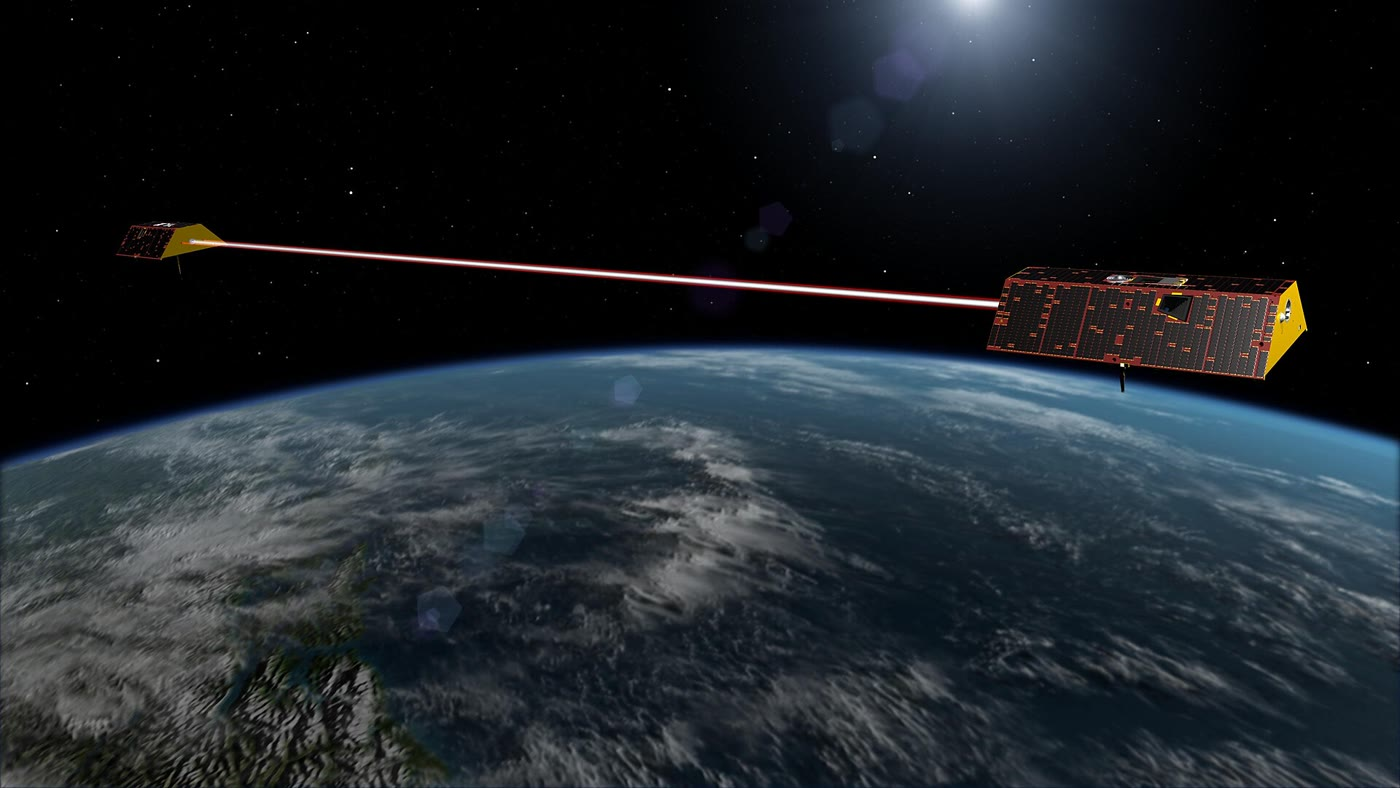
\includegraphics[width=0.66\linewidth]{images/book5/b3-grace-fo-concept.jpg}

\par\smallskip{\small दो ग्रेस फ़ॉलो-ऑन उपग्रह, एक कलाकार की दृष्टि से (उनके बीच की
दूरी बहुत कम दिखाई गई है)। लाल किरण लेज़र
परास-लिंक को दर्शाती है। NASA/JPL-Caltech, सार्वजनिक डोमेन।}
\label{fig:b3:gravity-geodesy:grace-photo}
\end{omfigure}

\begin{definition}[तुल्य जल-ऊँचाई]\label{def:b3:gravity-geodesy:ewh}
गुरुत्व क्षेत्र में ऐसा परिवर्तन, जो उस परत की मोटाई से कहीं अधिक दूरियों पर
धीरे-धीरे बदलता है, जिसमें द्रव्यमान स्थानांतरित हुआ, उसे पृथ्वी की सतह पर एक पतले खोल पर
पृष्ठ घनत्व $\sigma$ (\unit{kg.m^{-2}}) के परिवर्तन द्वारा निरूपित किया जा सकता है।
\emph{तुल्य जल-ऊँचाई}\index{तुल्य जल-ऊँचाई} उतने ही पृष्ठ घनत्व वाले मीठे पानी की
मोटाई है:
\[
  h_w = \frac{\sigma}{\rho_w} .
\]
\end{definition}

एक मीटर पानी का, \qty{1e6}{km^2} क्षेत्रफल वाले बेसिन पर, द्रव्यमान \qty{1e15}{kg} होता है, या
\qty{1000}{Gt}। समुद्र-तल लेखा-बही की दूसरी ओर है: \qty{360}{Gt} बर्फ़
महासागर में जुड़कर उसे लगभग एक मिलीमीटर ऊपर उठा देती है।
% ledger: data:b5-imbie
\omterm{def:b3:gravity-geodesy:satgrav}{उपग्रह गुरुत्वमिति}, उपग्रह ऊँचाईमापन, और हिमपात के संतुलन बनाम हिम-निर्वहन,
इनमें से हर एक हिमचादरों का द्रव्यमान संतुलन मापता है; इन्हें मिलाने पर
नीचे दी गई श्रेणी प्राप्त होती है।

\begin{omfigure}
\begin{tikzpicture}
\begin{axis}[omrecord, width=0.82\linewidth, height=0.5\linewidth,
  xmin=1992, xmax=2021, ymin=-5600, ymax=600,
  xlabel={वर्ष}, ylabel={संचयी द्रव्यमान परिवर्तन (\unit{Gt})},
  xticklabel style={/pgf/number format/1000 sep={}},
  legend pos=south west, legend cell align=left, legend style={font=\scriptsize}]
\addplot[name path=gl, draw=none, forget plot] table[x=year, y=lo] {figdata/out/bachelor-3-ice_mass-greenland.dat};
\addplot[name path=gh, draw=none, forget plot] table[x=year, y=hi] {figdata/out/bachelor-3-ice_mass-greenland.dat};
\addplot[blue!25, forget plot] fill between[of=gl and gh];
\addplot[name path=al, draw=none, forget plot] table[x=year, y=lo] {figdata/out/bachelor-3-ice_mass-antarctica.dat};
\addplot[name path=ah, draw=none, forget plot] table[x=year, y=hi] {figdata/out/bachelor-3-ice_mass-antarctica.dat};
\addplot[red!20, forget plot] fill between[of=al and ah];
\addplot[blue!70!black, thick] table[x=year, y=cum] {figdata/out/bachelor-3-ice_mass-greenland.dat};
\addlegendentry{ग्रीनलैंड}
\addplot[red!70!black, thick] table[x=year, y=cum] {figdata/out/bachelor-3-ice_mass-antarctica.dat};
\addlegendentry{अंटार्कटिका}
\draw[gray, densely dotted] (axis cs:2002.25,-5600) -- (axis cs:2002.25,600);
\draw[gray, densely dotted] (axis cs:2017.5,-5600) -- (axis cs:2017.5,600);
\node[font=\scriptsize, gray!40!black, anchor=north] at (axis cs:2009.9,550) {ग्रेस वर्ष};
\end{axis}
\end{tikzpicture}

\par\smallskip{\small 1992 से ग्रीनलैंड और अंटार्कटिका की हिमचादरों का संचयी द्रव्यमान
परिवर्तन, एक-मानक-विचलन पट्टियों के साथ (आईएमबीआईई 2021 के मिलाए गए
अनुमान, ऊँचाईमापन, गुरुत्वमिति और इनपुट--आउटपुट विधि से)। 2020 के अंत तक
ग्रीनलैंड ने $\num{4890} \pm \qty{460}{Gt}$ और अंटार्कटिका ने
$\num{2670} \pm \qty{530}{Gt}$ खोया; सरल-रेखा फ़िट
1992--2020 पर \qty{-176}{Gt.yr^{-1}} और \qty{-91}{Gt.yr^{-1}} देते हैं, और
ग्रेस वर्षों पर \qty{-246}{Gt.yr^{-1}} और \qty{-127}{Gt.yr^{-1}} देते हैं।}
\label{fig:b3:gravity-geodesy:ice-mass}
\end{omfigure}

पृथ्वी की सतह पर मापी गई गुरुत्व विसंगति हार्मोनिक्स का योग होती है; उपग्रह की
ऊँचाई पर हर हार्मोनिक एक ऐसे गुणक द्वारा क्षीण होता है जो
उसकी तरंगदैर्घ्य पर निर्भर करता है।

\begin{proposition}[ऊर्ध्वगामी सांतत्य]\label{prop:b3:gravity-geodesy:upward}
उन द्रव्यमानों के ऊपर, जो इसे उत्पन्न करते हैं, सतह के साथ
$\Delta g_0\cos kx$ के रूप में बदलने वाली गुरुत्व विसंगति, जहाँ $k = 2\pi/\lambda$, ऊँचाई $z$ पर
(उसका \emph{ऊर्ध्वगामी सांतत्य}\index{ऊर्ध्वगामी सांतत्य}) होती है
\[
  \Delta g(x, z) = \Delta g_0\,e^{-kz}\cos kx .
\]
\end{proposition}

\begin{proof}
द्रव्यमानों के ऊपर विसंगति-विभव, और उसके साथ विसंगति, लाप्लास
समीकरण $\partial_x^2\Delta g + \partial_z^2\Delta g = 0$ को संतुष्ट करते हैं। चरों को पृथक करने पर
$\Delta g = Z(z)\cos kx$, जहाँ $Z'' = k^2Z$ है;
$z \to \infty$ की ओर सीमित रहने वाला हल $Z = \Delta g_0e^{-kz}$ है।
\end{proof}

\qty{400}{km} ऊँचाई पर \qty{1000}{km} लंबी विसंगति अपने आयाम का \qty{8}{\percent}
बनाए रखती है, और \qty{100}{km} लंबी लगभग उसका \num{1e-11} भाग;
उपग्रह लंबी तरंगदैर्घ्य देखते हैं, और सतह के सर्वेक्षण छोटी।

\section{स्थलमंडलीय आनमन}

पुस्तक 3 (स्नातक वर्ष 1) में भार की प्रतिपूर्ति स्थानीय रूप से मानी गई थी, जिसमें हर स्तंभ अपने ही सहारे तैरता है।
महासागरीय प्लेट पर स्थित ज्वालामुखी की प्रतिपूर्ति केवल अपने ही नीचे नहीं होती:
प्लेट उसके नीचे सैकड़ों किलोमीटर की चौड़ाई में मुड़ती है, और ज्वालामुखी के चारों ओर का समुद्री तल
एक खाई में धँस जाता है, जिसके परे वह एक निचले मेहराब में उठता है।

\begin{definition}[स्थलमंडलीय आनमन, आनमन दृढ़ता, प्रभावी प्रत्यास्थ मोटाई]\label{def:b3:gravity-geodesy:flexure}
\emph{स्थलमंडलीय आनमन}\index{स्थलमंडलीय आनमन} भार के नीचे स्थलमंडल का मुड़ना है,
जिसे एक पतली प्रत्यास्थ प्लेट के मुड़ने के रूप में प्रतिरूपित किया जाता है,
जो एक तरल प्रावार पर तैरती है। प्लेट के मुड़ने का प्रतिरोध उसकी
\emph{आनमन दृढ़ता}\index{आनमन दृढ़ता} है
\[
  D = \frac{ET_e^3}{12(1 - \nu^2)},
\]
और वह एकसमान प्रत्यास्थ प्लेट की मोटाई $T_e$, जो वास्तविक स्थलमंडल की तरह मुड़ती है,
उसकी \emph{प्रभावी प्रत्यास्थ मोटाई}\index{प्रभावी प्रत्यास्थ मोटाई} है।
\end{definition}

\begin{theorem}[पतली प्लेट का आनमन]\label{thm:b3:gravity-geodesy:plate}
दृढ़ता $D$ की एक पतली प्रत्यास्थ प्लेट, जो एक दिशा में प्रति इकाई क्षेत्रफल भार $q(x)$ से मुड़ती है,
$w(x)$ से नीचे विक्षेपित होती है और घनत्व $\rho_m$ के प्रावार पर तैरती है,
जिसकी खोखली जगह घनत्व $\rho_i$ की सामग्री से भरी है, वह
\emph{आनमन समीकरण}\index{आनमन समीकरण} का पालन करती है
\[
  D\frac{\mathrm d^4w}{\mathrm dx^4} + (\rho_m - \rho_i)g\,w = q(x) .
\]
\end{theorem}

\begin{proof}
मुड़ी हुई प्लेट में मध्य-तल के ऊपर के तंतु संकुचित होते हैं और नीचे के
विस्तारित होते हैं, जो वक्रता $w''$ के अनुपात में है; मोड़ने वाले प्रतिबल का
मोटाई पर समाकलन करने से मोड़ आघूर्ण $M = -Dw''$ प्राप्त होता है, परिभाषा की दृढ़ता के साथ
(प्लेट बग़ल में फैल नहीं सकती, इसलिए गुणक
$1 - \nu^2$ आता है; भौतिकी की पुस्तकें, स्नातक वर्ष 3 का खंड देखिए)। प्लेट का एक टुकड़ा $\mathrm dx$
अपने फलकों पर कर्तन बल $V$ और आघूर्ण $M$ वहन करता है। ऊर्ध्वाधर संतुलन:
नीचे की ओर भार $q\,\mathrm dx$ और ऊपर की ओर विस्थापित प्रावार की उत्प्लावकता
$(\rho_m - \rho_i)gw\,\mathrm dx$ मिलकर $\mathrm dV/\mathrm dx = -q +
(\rho_m - \rho_i)gw$ देते हैं। आघूर्ण संतुलन से $\mathrm dM/\mathrm dx = V$ प्राप्त होता है।
तब $-Dw'''' = M'' = V' = -q + (\rho_m - \rho_i)gw$।
\end{proof}

\begin{definition}[आनमन प्राचल, अग्र-उभार]\label{def:b3:gravity-geodesy:alpha}
किसी प्लेट का \emph{आनमन प्राचल}\index{आनमन प्राचल} वह
लंबाई है
\[
  \alpha = \left(\frac{4D}{(\rho_m - \rho_i)g}\right)^{1/4},
\]
जो उसके आनमन का क्षैतिज पैमाना तय करती है। \emph{अग्र-उभार}\index{अग्र-उभार}
ऊपर की ओर के आनमन का वह निचला मेहराब है, जिसे मुड़ी प्लेट अपने भार के पास की खाई या
द्रोणी के परे उठाती है।
\end{definition}

\begin{proposition}[सतत प्लेट पर रेखीय भार]\label{prop:b3:gravity-geodesy:line}
$V_0$ प्रति इकाई लंबाई का रेखीय भार, जो $x = 0$ के साथ है, प्लेट को
\[
  w(x) = w_0e^{-|x|/\alpha}\left(\cos\frac{|x|}{\alpha} + \sin\frac{|x|}{\alpha}\right),
  \qquad w_0 = \frac{V_0\alpha^3}{8D} .
\]
विक्षेपित करता है। विक्षेपण $|x| = 3\pi\alpha/4$ पर शून्य होता है, जो खाई का किनारा है; \omterm{def:b3:gravity-geodesy:alpha}{अग्र-उभार} का
शिखर $|x| = \pi\alpha$ पर है, जिसकी ऊँचाई $w_0e^{-\pi} =
\num{0.0432}\,w_0$ है। संपूर्ण विक्षेपण की उत्प्लावकता भार को संतुलित करती है:
$\int(\rho_m - \rho_i)gw\,\mathrm dx = V_0$।
\end{proposition}

\begin{proof}
$x > 0$ के लिए समीकरण $w'''' + 4w/\alpha^4 = 0$ है; इसके सहायक समीकरण के मूल
$r^4 = -4/\alpha^4$ के मूल $(\pm1 \pm i)/\alpha$ हैं, और दूर पर शून्य होने वाले हल
$e^{-x/\alpha}(A\cos(x/\alpha) + B\sin(x/\alpha))$ हैं। समरूपता से
$w'(0) = 0$ का नियम बनता है, जिससे $A = B = w_0$ आता है। भार के पार ऊर्ध्वाधर संतुलन का समाकलन करने पर
कर्तन बल $V = -Dw'''$ में $-V_0$ की छलाँग आती है; समरूपता से
$w'''(0^-) = -w'''(0^+)$, और $w'''(0^+) = 4w_0/\alpha^3$, इसलिए $8Dw_0/\alpha^3 =
V_0$। विक्षेपण वहाँ शून्य होता है जहाँ $\tan(x/\alpha) =
-1$ है, पहली बार $x = 3\pi\alpha/4$ पर; इसका अवकलज,
$-(2w_0/\alpha)e^{-x/\alpha}\sin(x/\alpha)$, अगली बार $x = \pi\alpha$ पर शून्य होता है।
अंत में $\int_0^\infty e^{-u}(\cos u + \sin u)\,\mathrm du = 1$, इसलिए
$\int w\,\mathrm dx = 2w_0\alpha = V_0\alpha^4/(4D) = V_0/((\rho_m - \rho_i)g)$।
\end{proof}

\begin{proposition}[टूटी हुई प्लेट]\label{prop:b3:gravity-geodesy:broken}
$x = 0$ पर टूटी और अपने मुक्त सिरे पर नीचे दबाई गई प्लेट, जैसे गहरे समुद्र की
खाई पर $w = w_0e^{-x/\alpha}\cos(x/\alpha)$ की तरह, $x \ge 0$ के लिए, विक्षेपित होती है:
विक्षेपण $x = \pi\alpha/2$ पर शून्य होता है, और \omterm{def:b3:gravity-geodesy:alpha}{अग्र-उभार} का शिखर, यानी बाहरी उठाव,
$x = 3\pi\alpha/4$ पर है, जिसकी ऊँचाई $w_0e^{-3\pi/4}/\sqrt2 =
\num{0.067}\,w_0$ है।
\end{proposition}

\begin{proof}
वही क्षयकारी हल, इस अंतर के साथ कि मुक्त सिरा कोई आघूर्ण वहन नहीं करता,
$w''(0) = 0$ से $B = 0$ आता है। शून्य $\cos(x/\alpha) = 0$ पर है; अवकलज
$-(w_0/\alpha)e^{-x/\alpha}(\cos + \sin)(x/\alpha)$ $x = 3\pi\alpha/4$ पर शून्य होता है,
जहाँ $w = w_0e^{-3\pi/4}\cos(3\pi/4)$।
\end{proof}

इस प्रकार दूरियाँ प्लेट की मज़बूती की कुंजी हैं: खाई जहाँ समाप्त होती है
या उभार का शिखर जहाँ है, वह मापिए, तो $\alpha$ मिलता है, फिर $D$, और फिर $T_e$।
चूँकि $T_e$, $\alpha^{4/3}$ के रूप में आता है, दूरी का एक उचित अनुमान
मोटाई का एक अच्छा अनुमान देता है।

\begin{omfigure}
\begin{tikzpicture}
\begin{groupplot}[group style={group size=1 by 2, vertical sep=1.5cm},
  width=0.82\linewidth, height=0.36\linewidth, xmin=-400, xmax=400,
  tick label style={font=\scriptsize}, label style={font=\small}, title style={font=\small}]
\nextgroupplot[title={(क) रेखीय भार: तीन मोटाइयों की प्लेटों पर ओरू कटक},
  ylabel={विक्षेपण (\unit{m})}, ymin=-3000, ymax=700, y filter/.expression={-y},
  legend pos=south east, legend cell align=left, legend style={font=\scriptsize}]
\addplot[red!70!black, thick] table[x=x, y=w10] {figdata/out/bachelor-3-flexure-profiles.dat};
\addlegendentry{$T_e = \qty{10}{km}$}
\addplot[blue!70!black, thick] table[x=x, y=w25] {figdata/out/bachelor-3-flexure-profiles.dat};
\addlegendentry{$T_e = \qty{25}{km}$}
\addplot[green!45!black, thick] table[x=x, y=w40] {figdata/out/bachelor-3-flexure-profiles.dat};
\addlegendentry{$T_e = \qty{40}{km}$}
\draw[gray] (axis cs:-400,0) -- (axis cs:400,0);
\draw[->, blue!70!black] (axis cs:222,330) -- (axis cs:222,90);
\node[font=\scriptsize, blue!70!black, anchor=south] at (axis cs:222,330) {अग्र-उभार, $\pi\alpha$};
\nextgroupplot[title={(ख) खाई पर टूटी प्लेट, $T_e = \qty{25}{km}$},
  xlabel={भार या खाई से दूरी (\unit{km})},
  ylabel={विक्षेपण (\unit{m})}, xmin=0, xmax=400, ymin=-1100, ymax=280,
  y filter/.expression={-y}]
\addplot[blue!70!black, thick] table[x=x, y=w] {figdata/out/bachelor-3-flexure-broken.dat};
\draw[gray] (axis cs:0,0) -- (axis cs:400,0);
\draw[->] (axis cs:166.5,200) -- (axis cs:166.5,80);
\node[font=\scriptsize, anchor=west] at (axis cs:170,200) {बाहरी उठाव, $3\pi\alpha/4$};
\end{groupplot}
\end{tikzpicture}

\par\smallskip{\small लोचदार प्लेट का आनमन (परिकलित;
$E = \qty{100}{GPa}$, $\nu = 0.25$, प्रावार \qty{3300}{kg.m^{-3}}, खाई में
जल; ऊर्ध्वाधर पैमाना बहुत बढ़ाकर दिखाया गया)। (क) ज्वालामुखी
कटक के भार (\qty{4.17e12}{N.m^{-1}}) के नीचे पतली प्लेट गहरी और संकरी धँसती है, मोटी
उथली और चौड़ी; \omterm{def:b3:gravity-geodesy:alpha}{अग्र-उभार} \qty{112}{km} से
\qty{316}{km} तक खिसकता है। (ख) खाई पर टूटी प्लेट, जो \qty{1}{km} नीचे दबाई गई है:
बाहरी उठाव खाई से \qty{167}{km} दूर \qty{67}{m} ऊँचा है।}
\label{fig:b3:gravity-geodesy:flexure}
\end{omfigure}

\begin{definition}[क्षेत्रीय समस्थितिक प्रतिपूर्ति]\label{def:b3:gravity-geodesy:regional}
\emph{क्षेत्रीय समस्थितिक प्रतिपूर्ति}\index{क्षेत्रीय समस्थितिक प्रतिपूर्ति}
किसी भार का सहारा उस विक्षेपण की उत्प्लावकता से मिलता है, जो
भार से चौड़े क्षेत्र में फैला हो, स्थलमंडल की मोड़ सामर्थ्य के माध्यम से; इसके विपरीत एयरी
या प्रैट प्रतिपूर्ति में प्रत्येक स्तंभ अपने ही नीचे प्रतिपूरित होता है।
\end{definition}

स्थानीय और क्षेत्रीय प्रतिपूर्ति एक ही कुल द्रव्यमान को संतुलित करती हैं, परंतु
उसे अलग ढंग से वितरित करती हैं: कठोर प्लेट पर संकरे भार के नीचे मूल उथला और चौड़ा होता है,
और भार के ऊपर गुरुत्व विसंगति अत्यधिक धनात्मक होती है, जिसके दोनों ओर ऋणात्मक
विसंगतियाँ खाई के ऊपर होती हैं। हवाई कटक के द्वीपों के आसपास गुरुत्व और
भूकंपीय परिच्छेद 17 से \qty{37}{km} तक प्रभावी प्रत्यास्थ मोटाइयाँ देते हैं, और
एम्परर श्रृंखला के प्राचीन समुद्री पर्वतों के साथ 10 से \qty{20}{km} तक, यह अंतर
ज्वालामुखियों और जिस प्लेट पर उन्होंने भार डाला, उनकी आयु से अपेक्षित है;
ये मान ठंडी हो रही महासागरीय प्लेट में, लगभग
\qty{350}{\degreeCelsius} की समतापरेखा की गहराई का अनुसरण करते हैं।
% ledger: watts25:te
पर्वत पट्टी के भार के नीचे वही मोड़
अग्रभूमि द्रोणियाँ खोलता है; इसका विवरण पुस्तक 4 (स्नातक वर्ष 2) में ऐल्पाइन पर्वतजनक पट्टी वाले अध्याय में है।

\begin{omfigure}
\begin{tikzpicture}[font=\scriptsize, x=1cm, y=1cm]
\fill[blue!8] (-6,0) rectangle (6,-1.0);
\draw[blue!50!black] (-6,0) -- (6,0) node[right] {समुद्र-तल};
% volcano
\fill[brown!45] (-1.2,-1.6) -- (0,0.5) -- (1.2,-1.6) -- cycle;
% moat infill
\fill[yellow!35] (-1.2,-1.6) .. controls (-2.0,-1.5) and (-3.0,-1.15) .. (-3.6,-1.02) -- (-1.2,-1.02) -- cycle;
\fill[yellow!35] (1.2,-1.6) .. controls (2.0,-1.5) and (3.0,-1.15) .. (3.6,-1.02) -- (1.2,-1.02) -- cycle;
% flexed seafloor (top of crust)
\draw[very thick, brown!60!black] (-6,-0.96) .. controls (-5.2,-0.78) and (-4.4,-0.78) .. (-3.6,-1.02)
  .. controls (-3.0,-1.15) and (-2.0,-1.5) .. (-1.2,-1.6) -- (1.2,-1.6)
  .. controls (2.0,-1.5) and (3.0,-1.15) .. (3.6,-1.02) .. controls (4.4,-0.78) and (5.2,-0.78) .. (6,-0.96);
% Moho, parallel
\draw[thick, gray!60!black] (-6,-1.76) .. controls (-5.2,-1.58) and (-4.4,-1.58) .. (-3.6,-1.82)
  .. controls (-3.0,-1.95) and (-2.0,-2.3) .. (-1.2,-2.4) -- (1.2,-2.4)
  .. controls (2.0,-2.3) and (3.0,-1.95) .. (3.6,-1.82) .. controls (4.4,-1.58) and (5.2,-1.58) .. (6,-1.76);
\node[anchor=west] at (4.2,-1.95) {मोहो};
\draw[dashed, gray] (-6,-1.0) -- (6,-1.0);
\node[anchor=north west, gray!40!black] at (-6,-1.03) {बिना मुड़ा समुद्र-तल};
\node[anchor=south, align=center] at (-2.6,-0.98) {खाई\\(भराव)};
\node[anchor=south] at (4.8,-0.82) {अग्र-उभार};
\node at (0,-0.6) {ज्वालामुखी};
\node[anchor=north] at (0,-2.5) {कुछ $\alpha$ चौड़ाई पर नीचे मुड़ी प्लेट};
\end{tikzpicture}

\par\smallskip{\small महासागरीय प्लेट पर एक ज्वालामुखीय द्वीप (योजनाबद्ध
अनुप्रस्थ काट, ऊर्ध्वाधर पैमाना बढ़ाकर दिखाया गया)। प्लेट ज्वालामुखी के नीचे मुड़ती है;
उसके चारों ओर का गड्ढा, यानी खाई, ज्वालामुखीय मलबे और अवसाद से भरता है, और
उसके परे प्लेट एक निम्न \omterm{def:b3:gravity-geodesy:alpha}{अग्र-उभार} में ऊपर उठती है।}
\label{fig:b3:gravity-geodesy:moat}
\end{omfigure}

\begin{inthefield}[सापेक्ष गुरुत्व सर्वेक्षण]
\begin{minipage}[t]{0.55\linewidth}\vspace{0pt}
निरपेक्ष गुरुत्वमापी एक निर्वात कक्ष में कोना-घन दर्पण गिराता है,
बार-बार और उसके गिरने का समय लेज़र इंटरफ़ेरोमीटर और परमाणु घड़ी से मापता है;
यह एक स्टेशन पर गुरुत्व ज्ञात करता है, परंतु यह भारी है और स्थापित करने में धीमा है।
सर्वेक्षण स्वयं एक सापेक्ष गुरुत्वमापी से होता है, एक छोटा स्प्रिंग-तुला,
जो गुरुत्व के अंतर मापता है। भूभौतिकीविद् रेखा के प्रत्येक
स्टेशन पर इसे आधार-प्लेट पर समतल करता है, पढ़ता है, समय और ऊँचाई दर्ज करता है, और आगे बढ़ता है; हर
कुछ घंटों पर लूप किसी आधार स्टेशन पर लौटता है, ताकि स्प्रिंग का धीमा बहाव
और ठोस पृथ्वी के ज्वार मापे और हटाए जा सकें। एक उपग्रह
ग्राही, पास के एक दंड पर, स्थिति और ऊँचाई देता है, क्योंकि गुरुत्व
हर मीटर ऊँचाई के लिए लगभग \qty{0.3}{\milli\gal} बदलता है।
\end{minipage}\hfill
\begin{minipage}[t]{0.42\linewidth}\vspace{0pt}
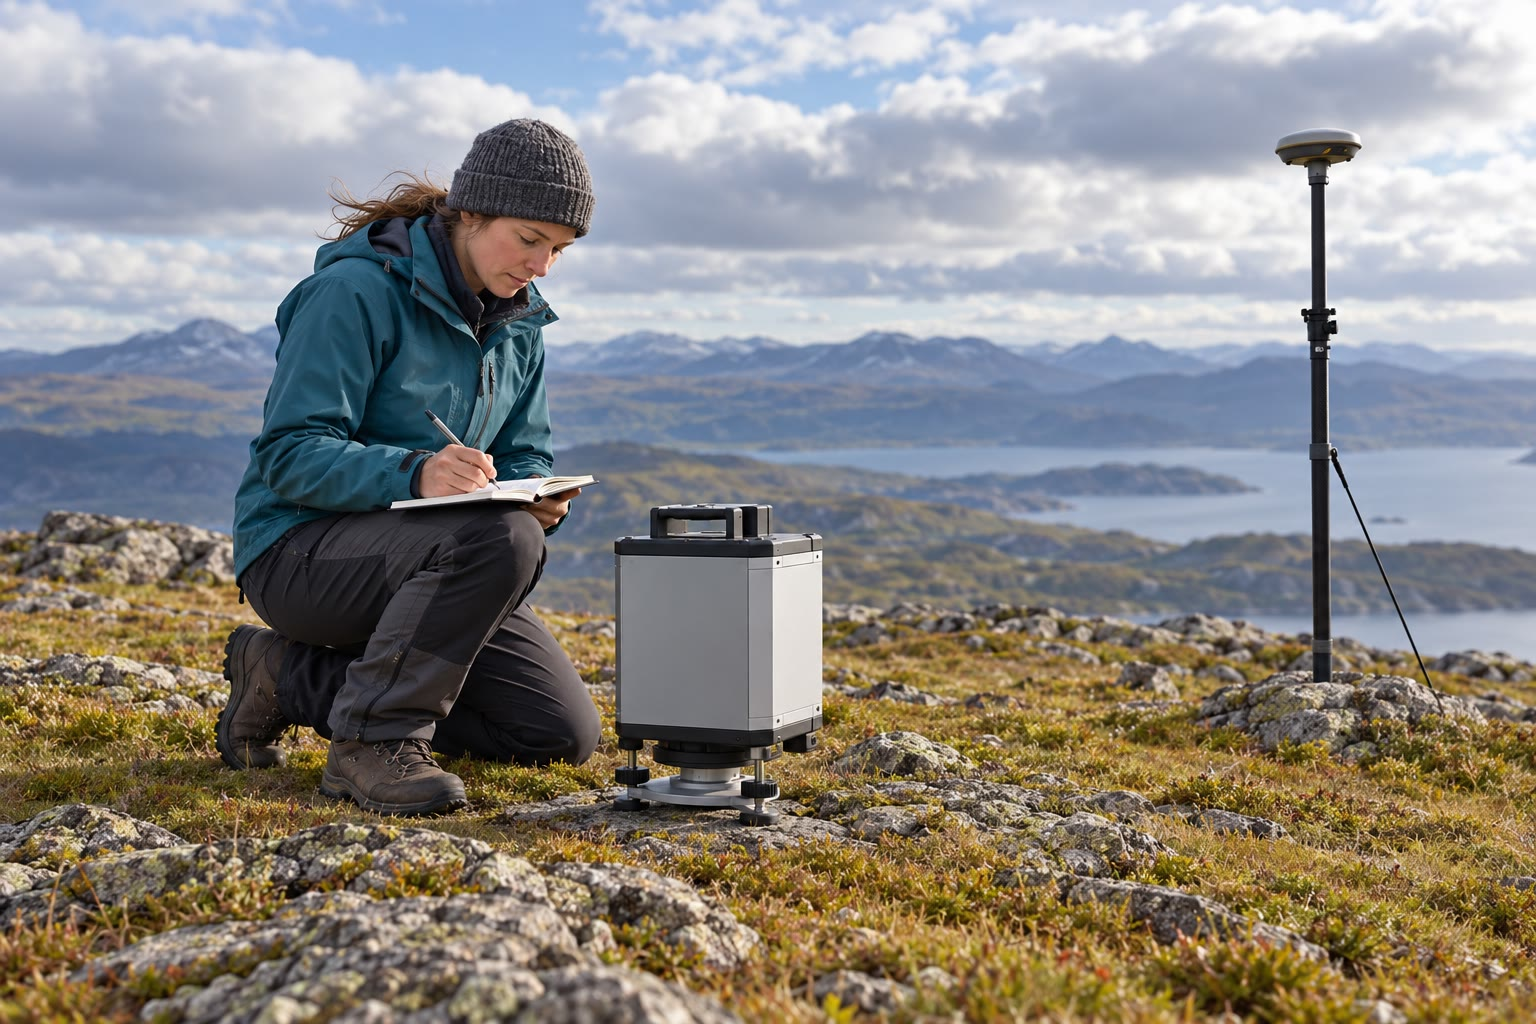
\includegraphics[width=\linewidth]{images/book5/ai/b3-gravimeter.jpg}

{\scriptsize समतलन आधार पर एक क्षेत्रीय गुरुत्वमापी, जिसके पीछे उपग्रह
एंटीना दिख रहा है (AI से बनाया गया चित्रण)।}
\end{minipage}
\end{inthefield}

\section{अभ्यास}

\begin{exercise}[$\star$]\label{exo:b3:gravity-geodesy:1}
भूगणितीय संदर्भ तंत्र 1980 के मान $a = \qty{6378137}{m}$ और
$f = \num{0.00335281068}$ लेकर लघु अर्ध-अक्ष $b$ और $a - b$ परिकलित कीजिए।
$J_2 = \num{1.08263e-3}$ और $m = \num{0.00344979}$ लेकर, क्लेरो संबंध
द्वारा पूर्वानुमानित चपटापन परिकलित कीजिए, और तुलना कीजिए।
\end{exercise}

\begin{exercise}[$\star$]\label{exo:b3:gravity-geodesy:2}
एक शुष्क वर्ष में \qty{5.0e5}{km^2} की एक नदी द्रोणी
\qty{60}{Gt} जल खो देती है। \omterm{def:b3:gravity-geodesy:ewh}{तुल्य जल-ऊँचाई} में परिवर्तन परिकलित कीजिए। वही द्रव्यमान
समुद्र-तल को कितना ऊपर उठा देगा, \qty{360}{Gt} प्रति मिलीमीटर मानकर?
\end{exercise}

\begin{exercise}[$\star$]\label{exo:b3:gravity-geodesy:3}
श्रेणी $\gamma = 9.780327(1 + 0.0053024\sin^2\varphi -
0.0000058\sin^22\varphi)$ \unit{m.s^{-2}} लेकर, विषुवत रेखा पर,
\ang{45} और ध्रुवों पर सामान्य गुरुत्व परिकलित कीजिए। ध्रुव और विषुवत रेखा के बीच
का अंतर मिलीगैल में व्यक्त कीजिए।
\end{exercise}

\begin{exercise}[$\star$]\label{exo:b3:gravity-geodesy:4}
महासागरीय प्लेटों की \omterm{def:b3:gravity-geodesy:flexure}{आनमन दृढ़ता} और \omterm{def:b3:gravity-geodesy:alpha}{आनमन प्राचल} परिकलित कीजिए, जिनके लिए
$T_e = \qty{10}{km}$ और $T_e = \qty{30}{km}$ हैं ($E = \qty{100}{GPa}$,
$\nu = 0.25$, $\rho_m - \rho_w = \qty{2270}{kg.m^{-3}}$, $g =
\qty{9.81}{m.s^{-2}}$)। एक रेखीय भार के नीचे खाई का किनारा और \omterm{def:b3:gravity-geodesy:alpha}{अग्र-उभार}
कहाँ स्थित होते हैं?
\end{exercise}

\begin{exercise}[$\star\star$]\label{exo:b3:gravity-geodesy:5}
(क) जियॉइड ऊँचाई $+\qty{50}{m}$ होने पर वहाँ विक्षोभी विभव परिकलित कीजिए,
$\gamma = \qty{9.80}{m.s^{-2}}$ लेते हुए। (ख) \qty{100}{km} की दूरी पर जियॉइड
\qty{10}{m} ऊपर उठता है। वहाँ साहुल रेखा दीर्घवृत्तज के अभिलंब से
किस कोण से भिन्न होती है? उसे चाप-सेकंड में व्यक्त कीजिए।
\end{exercise}

\begin{exercise}[$\star\star$]\label{exo:b3:gravity-geodesy:6}
$J_2 = \num{1.08263e-3}$ और जड़त्व-आघूर्ण गुणक
$C/(Ma^2) = \num{0.3308}$ से गतिक विलक्षणता $H = (C - A)/C$ और
$1/H$ परिकलित कीजिए। समान $J_2$ वाली एकसमान पृथ्वी इन दोनों में से कौन-सी संख्या बदलेगी?
\end{exercise}

\begin{exercise}[$\star\star$]\label{exo:b3:gravity-geodesy:7}
एक उपग्रह भूमध्यरेखीय त्रिज्या से \qty{500}{km} ऊपर की वृत्ताकार कक्षा में
चलता है ($a = \qty{6378.137}{km}$, $GM = \qty{3.986005e14}{m^3.s^{-2}}$), जिसका झुकाव \ang{89} है।
उसका आवर्तकाल और नोडल पुरस्सरण की दर प्रति दिन अंशों में परिकलित कीजिए।
गुरुत्व मिशन लगभग-ध्रुवीय कक्षाएँ क्यों चुनते हैं?
\end{exercise}

\begin{exercise}[$\star\star$]\label{exo:b3:gravity-geodesy:8}
सतह पर \qty{10}{\milli\gal} की दो गुरुत्व विसंगतियाँ हैं, जिनके तरंगदैर्घ्य
\qty{100}{km} और \qty{1000}{km} हैं। \qty{500}{km} ऊँचाई पर उनके आयाम
परिकलित कीजिए।
\end{exercise}

\begin{exercise}[$\star\star$]\label{exo:b3:gravity-geodesy:9}
खाई के समुद्र की ओर, बाहरी उभार का शिखर खाई-अक्ष से
\qty{120}{km} दूर स्थित है। प्लेट के ऊपर जल होने पर टूटी-प्लेट मॉडल लेते हुए,
$\alpha$, $D$ और $T_e$ तथा वह दूरी परिकलित कीजिए जहाँ प्लेट
अपने अनानमित स्तर को पार करती है।
\end{exercise}

\begin{exercise}[$\star\star\star$]\label{exo:b3:gravity-geodesy:10}
(क) जाँचिए कि $w = w_0e^{-u}(\cos u + \sin u)$, $u = x/\alpha$,
$Dw'''' + (\rho_m - \rho_i)gw = 0$ को $x > 0$ के लिए, $\alpha$ की परिभाषा के अनुसार, संतुष्ट करता है।
(ख) दिखाइए कि झुकाव आघूर्ण $-Dw''$ भार के नीचे सबसे अधिक होता है और
$x = \pi\alpha/4$ पर चिह्न बदलता है। (ग) प्लेट की ऊपरी सतह पर दरार
कहाँ सबसे संभावित है, और क्यों?
\end{exercise}

\begin{exercise}[$\star\star\star$]\label{exo:b3:gravity-geodesy:11}
$m = \num{0.00344979}$ और $C/(Ma^2) = \num{0.3308}$ लेकर, द्रवस्थैतिक चपटापन के लिए
डार्विन--रैडो संबंध को व्युत्क्रमित कीजिए।
$f = \num{0.00335281}$ से तुलना कीजिए: अंतर और द्रवस्थैतिक आकृति के ऊपर
भूमध्य रेखा की अतिरिक्त ऊँचाई परिकलित कीजिए। इससे प्रावार के बारे में क्या पता चलता है?
\end{exercise}

\begin{exercise}[$\star\star\star$]\label{exo:b3:gravity-geodesy:12}
\qty{700}{km} ऊँची वृत्ताकार कक्षा में एक उपग्रह को पूरे वर्ष सूर्य के सापेक्ष
एक ही अभिविन्यास बनाए रखना है: इसके लिए उसका नोड
\num{365.242}~दिन के एक उष्णकटिबंधीय वर्ष में \ang{360} आगे बढ़ना चाहिए। आवश्यक झुकाव परिकलित कीजिए।
\end{exercise}

\section{समस्या: ओरू कटक के चारों ओर की खाई}

\begin{problem}[{सप्ताहांत समस्या --- पृथ्वी की आकृति, एक ज्वालामुखीय भार,
उसकी आनमन खाई और उपग्रह उसमें क्या देखते हैं}]
\label{pb:b3:gravity-geodesy:1}
% values: calc/ch03.py; GRS80 (geod5:grs80-*), earth:MoI; flexure.py
ओरू महासागर में एक काल्पनिक ज्वालामुखीय कटक है: आपस में मिले ज्वालामुखियों की
\qty{400}{km} लंबी सीधी श्रृंखला, जो पुराने महासागरीय स्थलमंडल पर बनी है।
इसकी अनुप्रस्थ काट आधार पर \qty{80}{km} चौड़ा एक त्रिभुज मानी गई है और
\qty{6}{km} ऊँची है, जिसका घनत्व \qty{2800}{kg.m^{-3}} है, और जो
\qty{5}{km} गहरे समुद्र-तल पर खड़ी है। प्रावार का घनत्व \qty{3300}{kg.m^{-3}},
समुद्री जल का \qty{1030}{kg.m^{-3}}, $E = \qty{100}{GPa}$, $\nu = 0.25$, $g =
\qty{9.81}{m.s^{-2}}$, $G = \qty{6.674e-11}{m^3.kg^{-1}.s^{-2}}$.

\medskip
\noindent\textbf{भाग I --- पृथ्वी की आकृति।} भूगणितीय संदर्भ तंत्र
1980 का उपयोग कीजिए: $a = \qty{6378137}{m}$, $b = \qty{6356752.3}{m}$,
$GM = \qty{3.986005e14}{m^3.s^{-2}}$, $J_2 = \num{1.08263e-3}$,
$\omega = \qty{7.292115e-5}{rad.s^{-1}}$, $f = \num{0.00335281}$; और
$C/(Ma^2) = \num{0.3308}$।
\begin{enumerate}
  \item $m = \omega^2a^2b/(GM)$ परिकलित कीजिए।
  \item $J_2$ से क्लेरो संबंध द्वारा प्राप्त चपटापन
        $m$ की सहायता से और उसका व्युत्क्रम परिकलित कीजिए।
  \item डार्विन--रैडो संबंध से द्रवस्थैतिक चपटापन और उसका व्युत्क्रम
        परिकलित कीजिए।
  \item दोनों की प्रेक्षित चपटापन से तुलना कीजिए। द्रवस्थैतिक आकृति से
        भूमध्य रेखा कितने मीटर ऊपर उठी है?
  \item $H = (C - A)/C$ गतिक विलक्षणता परिकलित कीजिए।
\end{enumerate}

\noindent\textbf{भाग II --- भार।}
\begin{enumerate}[resume]
  \item कटक की अनुप्रस्थ काट का क्षेत्रफल परिकलित कीजिए।
  \item रेखीय भार $V_0$ परिकलित कीजिए। पूरे कटक को जलमग्न मानिए, ताकि
        उसका भार प्रति इकाई आयतन $(\rho_v - \rho_w)g$ हो।
  \item यदि कटक स्थानीय रूप से, एरी ढंग से, प्रावार में अपनी ही चट्टान की
        एक मूल द्वारा प्रतिपूर्ति पाता, तो शिखर के नीचे उस मूल की गहराई क्या
        होती?
  \item स्थानीय प्रतिपूर्ति के अंतर्गत मूल कटक के तल पर समाप्त होती,
        कटक की अक्ष से \qty{40}{km} दूर। बैथिमेट्री एक खाई दिखाती है, जो
        \qty{165}{km} तक फैली है। इससे आप क्या निष्कर्ष निकालते हैं?
\end{enumerate}

\noindent\textbf{भाग III --- आनमन खाई।} खाई जल से भरी है
($\rho_i = \rho_w$)। कटक के आर-पार एक भूकंपीय परिच्छेद में महासागरीय भूपर्पटी का ऊपरी भाग
अक्ष से \qty{165}{km} दूर अपनी क्षेत्रीय गहराई पर लौटती हुई पाई जाती है, और
\omterm{def:b3:gravity-geodesy:alpha}{अग्र-उभार} का शिखर अक्ष से \qty{220}{km} दूर पाया जाता है।
\begin{enumerate}[resume]
  \item खाई के किनारे से \omterm{def:b3:gravity-geodesy:alpha}{आनमन प्राचल} परिकलित कीजिए।
  \item \omterm{def:b3:gravity-geodesy:alpha}{अग्र-उभार} से उसे फिर से परिकलित कीजिए। क्या दोनों संगत हैं?
  \item $\alpha = \qty{70.0}{km}$ लेते हुए, \omterm{def:b3:gravity-geodesy:flexure}{आनमन दृढ़ता} परिकलित कीजिए।
  \item \omterm{def:b3:gravity-geodesy:flexure}{प्रभावी प्रत्यास्थ मोटाई} परिकलित कीजिए।
  \item $V_0 = \qty{4.17e12}{N.m^{-1}}$ और $D$ को तीन अंकों तक पूर्णांकित लेकर,
        अक्ष के नीचे विक्षेपण परिकलित कीजिए।
  \item \omterm{def:b3:gravity-geodesy:alpha}{अग्र-उभार} की ऊँचाई परिकलित कीजिए।
  \item जाँचिए कि संपूर्ण विक्षेपण की उत्प्लावकता, $2w_0\alpha(\rho_m -
        \rho_w)g$, $V_0$ को संतुलित करती है।
  \item हवाई कटक पर पाए गए मानों के साथ, 17 से
        \qty{37}{km} तक, $T_e$ की तुलना कीजिए। अक्ष के नीचे विक्षेपण की
        तुलना प्रश्न 8 के एरी मूल से कीजिए।
\end{enumerate}

\noindent\textbf{भाग IV --- खाई के ऊपर गुरुत्व।} आनमन की एक हार्मोनिक लीजिए, जिसका
तरंगदैर्घ्य $2\pi\alpha$ और आयाम $W = \qty{500}{m}$ है, और जो
समुद्र-तल (भूपर्पटी \qty{2900}{kg.m^{-3}}, जल के नीचे, समुद्र-तल से \qty{5}{km} नीचे)
और मोहो (भूपर्पटी के नीचे प्रावार, समुद्र-तल से \qty{12}{km} नीचे) दोनों को विक्षेपित करती है।
सतही घनत्व $\sigma$ की एक पतली परत $2\pi G\sigma$ की विसंगति
उसके ठीक ऊपर उत्पन्न करती है।
\begin{enumerate}[resume]
  \item हार्मोनिक का तरंगदैर्घ्य और तरंग-संख्या $k$ परिकलित कीजिए।
  \item \qty{5}{km} गहराई से \omterm{prop:b3:gravity-geodesy:upward}{ऊर्ध्वगामी सांतत्य} द्वारा समुद्र-तल तक लाए गए,
        विक्षेपित समुद्र-तल के कारण समुद्र-तल पर विसंगति का आयाम परिकलित कीजिए।
  \item विक्षेपित मोहो का आयाम, और कुल आयाम परिकलित कीजिए।
  \item समुद्र-तल से \qty{400}{km} ऊपर स्थित उपग्रह की ऊँचाई पर कुल विसंगति
        परिकलित कीजिए।
  \item कटक की चौड़ाई, \qty{80}{km} तरंगदैर्घ्य की एक हार्मोनिक, उस ऊँचाई पर
        किस गुणक से क्षीण होती है? उपग्रह क्या विभेदित कर सकता है?
  \item प्रश्न 18 की हार्मोनिक किस गोलीय-हार्मोनिक घात $n \approx 2\pi R/\lambda$ से
        संगत है ($R = \qty{6371}{km}$)?
  \item ओरू कटक के नीचे की प्लेट की \omterm{def:b3:gravity-geodesy:flexure}{प्रभावी प्रत्यास्थ मोटाई}
        ज्ञात कीजिए।
\end{enumerate}
\end{problem}
